% ---------------------------------------------------------------------------
% Scrum Roles
\begin{frame}
    \frametitle{Scrum Roles}
    \begin{columns}
        % Dr. Simon Kramer
        \column{0.25\textwidth}
        \centering
        
\includegraphics[width=0.45\linewidth]{../assets/avatar_placeholder.jpg} \\
        \textbf{Dr. Simon Kramer} \\ \small{Stakeholder} \par\vspace{0.5cm}
        % Dominic Gernert
        \column{0.25\textwidth}
        \centering
        
\includegraphics[width=0.45\linewidth]{../assets/avatar_placeholder.jpg} \\
        \textbf{Dominic Gernert} \\ \small{Product Owner} \par\vspace{0.5cm}
    \end{columns}
    \begin{columns}
        % Lukas von Allmen
        \column{0.25\textwidth}
        \centering
        
\includegraphics[width=0.45\linewidth]{../assets/avatar_placeholder.jpg} \\
        \textbf{Lukas von Allmen} \\ \small{Scrum Master}
        % Darius Degel
        \column{0.25\textwidth}
        \centering
        
\includegraphics[width=0.45\linewidth]{../assets/avatar_placeholder.jpg} \\
        \textbf{Darius Degel} \\ \small{Developer}
    \end{columns}
\end{frame}
% ---------------------------------------------------------------------------

% ---------------------------------------------------------------------------
% Backlog
\begin{frame}
    \frametitle{Backlog}
    \begin{columns}
        \column{0.5\textwidth}
        \begin{itemize}
            \large
            \item Epics \ensuremath{\approx} Labels
            \item Impediments
            \item Development Board
        \end{itemize}
        \column{0.5\textwidth}
        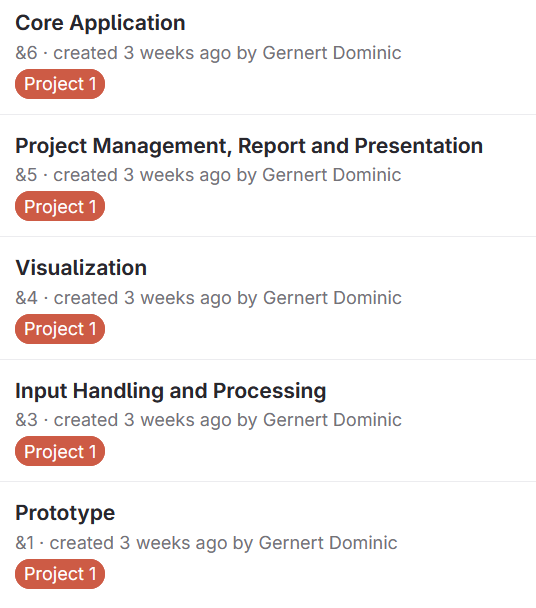
\includegraphics[width=0.8\linewidth]{../assets/epics_interim_presentation.png}
    \end{columns}
\end{frame}
% ---------------------------------------------------------------------------

% ---------------------------------------------------------------------------
% Backlog cont.
\begin{frame}
    \frametitle{Backlog}
    \centering
    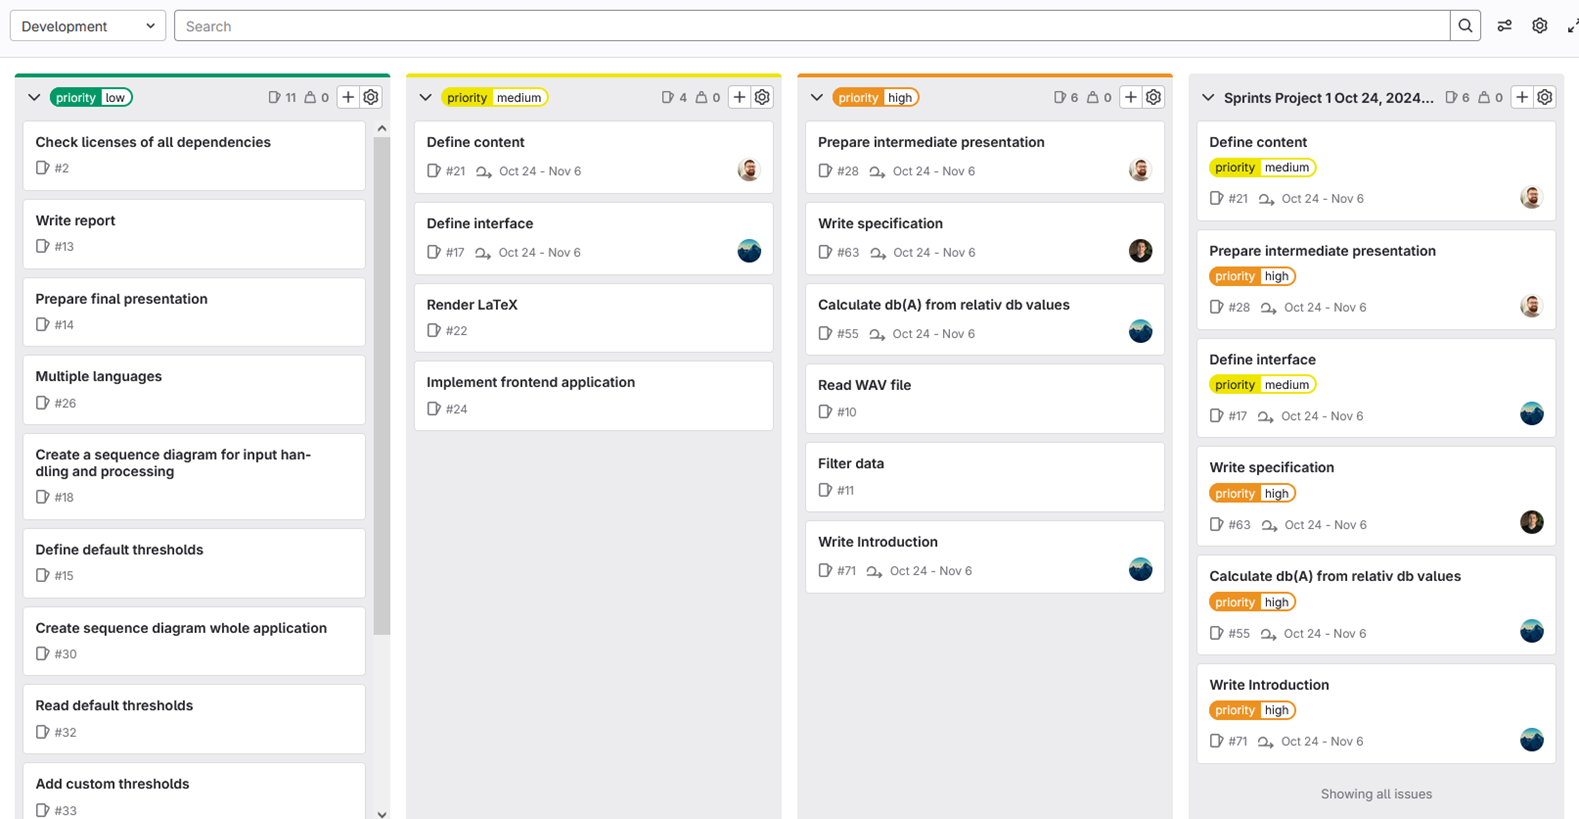
\includegraphics[width=0.85\linewidth]{../assets/backlog_interim_presentation.png}
\end{frame}
% ---------------------------------------------------------------------------

% ---------------------------------------------------------------------------
% Sprint Goals
\begin{frame}
    \frametitle{Sprint Goals}
    \begin{itemize}
        \large
        \item S.M.A.R.T
        \item Product Focus
    \end{itemize}
    \par\vspace{0.5cm}
    \begin{example}
        Prototypes with two different technologies are implemented and their pros and cons are evaluated.
    \end{example}
\end{frame}
% ---------------------------------------------------------------------------

% ---------------------------------------------------------------------------
% Review & Retro
\begin{frame}
    \frametitle{Review \& Retro}
    \centering
    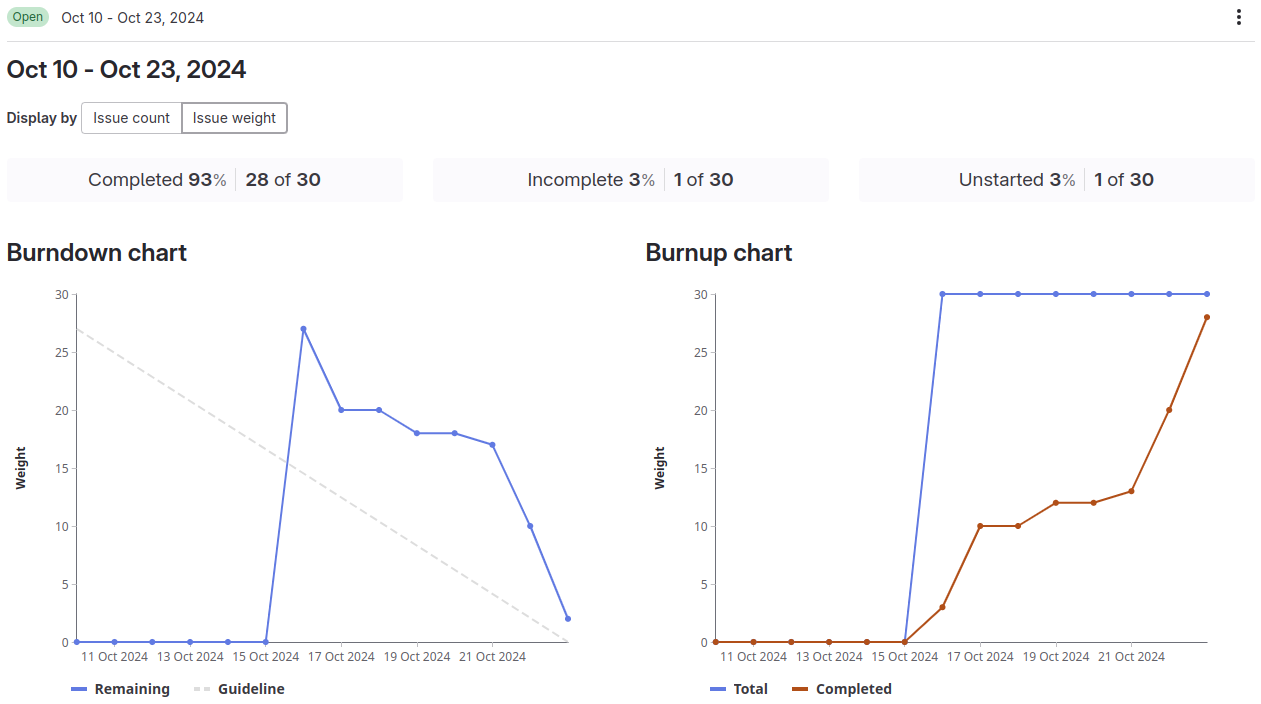
\includegraphics[width=0.84\linewidth]{../assets/burndown_sprint_001.png}
\end{frame}
% ---------------------------------------------------------------------------

% ---------------------------------------------------------------------------
% Review & Retro cont.
\begin{frame}
    \frametitle{Review \& Retro}
    \begin{columns}
        \column{0.5\textwidth}
        \large
        \textbf{Review}
        \begin{itemize}
            \large
            \item Demo
            \item Done / Not Done
            \item Goal Attainment
        \end{itemize}
        \column{0.5\textwidth}
        \large
        \textbf{Retro}
        \begin{itemize}
            \large
            \item What went well?
            \item What problems did we encounter?
            \item What are we improving in the future?
        \end{itemize}
    \end{columns}
\end{frame}
% ---------------------------------------------------------------------------

% ---------------------------------------------------------------------------
% Adaptations
\begin{frame}
    \frametitle{Adaptations}
    \begin{itemize}
        \large
        \item Product Owner
        \item Daily Scrum
        \item No Release Plan
        \item Retro
              \begin{itemize}
                  \large
                  \item Shorter first Retro
                  \item Successes, Problems, Improvements
              \end{itemize}
    \end{itemize}
\end{frame}
% ---------------------------------------------------------------------------